
\documentclass[12pt,a4paper]{report}
\usepackage{amsmath,amsthm,amssymb,graphicx,hyperref,float,mathalpha}
\usepackage[left=1.2in,right=1in,top=1in,bottom=1in]{geometry}
\usepackage[english]{babel}
\usepackage{color}
\usepackage{multirow}
\usepackage{listings}
\definecolor{mygreen}{rgb}{0,0.6,0}
\definecolor{mygray}{rgb}{0.5,0.5,0.5}
\definecolor{mymauve}{rgb}{0.58,0,0.82}
\definecolor{backcolour}{rgb}{0.95,0.95,0.92}

\lstset{ %
  backgroundcolor=\color{backcolour},   % choose the background color
  numberstyle=\tiny,
  basicstyle=\footnotesize,        % size of fonts used for the code
  breaklines=true,                 % automatic line breaking only at whitespace
  captionpos=b,                    % sets the caption-position to bottom
  commentstyle=\color{mygreen},    % comment style
  escapeinside={\%*}{*)},          % if you want to add LaTeX within your code
  keywordstyle=\color{blue},       % keyword style
  stringstyle=\color{mymauve},     % string literal style
  numbers=left,                    
  numbersep=5pt
}
\usepackage{comment}
\usepackage{hyperref}
\usepackage{amsmath}
\usepackage{amssymb}
\usepackage{multicol}
\usepackage{multirow}
\usepackage{algorithmic, algorithm}
\newcommand\tab[1][5mm]{\hspace*{#1}}

\begin{document}
\thispagestyle{empty}
\begin{center}
\begin{figure}[h!]
\vspace{-20pt}
\begin{center}

\includegraphics[width=100pt]{FMI-03.png}
\end{center}
\end{figure}

{\large{\bf UNIVERSITATEA DE VEST DIN TIMI\c SOARA

FACULTATEA DE MATEMATIC\u A \c SI INFORMATIC\u A}}

\vspace{65pt}
{\huge {\bf Verification of Binarized Neural Networks using alpha-beta-CROWN and Marabou}}

\vspace{65pt}
\end{center}

\noindent Rafael-Valentin Ban\\
\noindent Cosmin-\c Stefan Negureanu\\
\noindent Mihai-Iosif F\^{a}r\c tal\u a \hfill Conf. Dr. M\u ad\u alina Era\c scu\\
\noindent Cristina-Larisa Petcu\\
\noindent M\u ad\u alina-Maria Radu\\

\section*{Abstract}
\tab Neural networks are computational models inspired by the structure and functioning of the human brain. These networks are used in machine learning to recognize patterns, make predictions, or perform tasks by learning from data and are increasingly utilized in autonomous vehicles. 
One  example of  neural network is the German Traffic Sign Recognition Benchmark, which employs Neural Networks to analyze traffic signs. The tools we are focusing on are alpha-beta-CROWN, marabou, and nnenum. We managed to get results with Alpha-beta-CROWN while we could not  get Marabou to run properly and with Nnenum, it could not perform the Transpose and Sign operations that were included in the onnx files, and so we got exit\_codes instead of results.  The difficulty of the analysis of this benchmark arises from the wide range of angles, luminosity, distance, and colors, as well as the types of traffic signs that were photographed. The motivation of this project is to not only be able to reproduce the results from the VNNCompetition, but to try to solve penalties to increase the score of the benchmark used.


\tableofcontents

\chapter{Introduction}
\tab The International Verification of Neural Networks Competition (VNN-Comp) consists in the testing and comparison of different tools with multiple sets of data, from vast domains of acitvity. Such competitions offer an opportunity for the participants in the domain of Aritificial Intelligence to improve their knowledge and abilities as well as to contribute to the advancement of neural networks technologies. From these different domains and tools, we choose our desired tool and dataset.\\
\tab And so, we decided to choose the \textbf{Traffic Sign Recognition Benchmark}, because it is a problem that is ever present and which we all are confronted by in our day to day lives, a problem which needs an immediate solutions as the development and advancement of self-driving cars will require precise and constant recognition of different traffic signs. Solving this problem will bring a useful contribution in the efficiency of traffic management and the improvement of traffic safety. Traffic sign recognition is a safety tech system that recognizes traffic signs and relays the information displayed on the sign to the driver through the instrument cluster, information screen or heads-up display. Regarding the tools, we choose three: Alpha-Beta-CROWN, Marabou and Nnenum.\\
\tab Alpha-Beta-CROWN is a tool that checks neural networks, which are models used in automated learning. This tool uses efficient methods of calculation in order to offer inssurance that the neural network modes are robust and are immune to attacks and other problems. It can function efficiently, utilizing large volumes of data. In our experience, this was the only tool that we could successfully used and generate results with.\\
\tab The second tool that we chose, Marabou, is based on SMT technology which answers questions about the properties of a neural network. This tool accepts multiple entry formats, including protocol buffer files that are generated by the popular TensorFlow framework for neural networks. Unfortunately, in the end, this tool generated segmentation faults when giving it the data in the traffic sign recognition benchmark.\\
\tab After this setback, we decided to install and use the third tool, Nnenum, a tool for checking neural networks of high performance. It uses advanced abstractization for rapidly checking ReLU networks without sacrificing precisions. This tool is written in Python, utilizes GLPK for solving linear problems and directyl accepts ONNX files and VNNLIB property files. This tool, while having a better experience with, produced an out.csv file with exit codes instead of results. In the following chapters, we will present the dataset used for the traffic sign recognition benchmark, the three tools we used as well as the overall results obtained from each.

\chapter{Dataset description}
\tab The experiment we decided to tackle is the one presented in the paper \textbf{Architecturing Binarized Neural Networks for Traffic Sign Recognition} \cite{traffic_signs_paper}. The aforementioned experiment deals with \textbf{binarized neural networks} for traffic sign recognition. The paper discusses a bottom-up approach for designing BBNs by studying their constituent layer characteristics, like binarized convolutional layers, max pooling, batch normalization and fully connected layers. The authors of this paper study these aspects by exploring various combinations of the aforementioned layers with different kernel sizes, numerous filters and neurons using the \textbf{German Traffic Sign Recognition Benchmark} as training data.\\\\
\tab According to the paper, the \textbf{German Traffic Sign Recognition Benchmark} (\textbf{GTSRB}) is a multi-class single-image dataset that is used in the paper's experiment as training data for the BNNs. It consists of images of road signs of different types such as prohibitory signs ("No Entry", "Wrong Way", "Road Closed", "No Straight Ahead" and so on), danger signs ("Under Construction", "Do Not Cross", "Train Track", "Slippery Road" and so on), as well as mandatory signs ("Go Straight Ahead", "Turn Right", "Permitted Directions", "Buses / Trucks / Bicycles / Pedestrians Only" and more). The images in the dataset are of different sizes, with a range from 25 x 25 to 243 x 225, with some not being perfect squares. As a total count, it contains 39,209 images used for training and 12,630 used for the actual experiment.\\\\
\tab The diversity of the dataset does not end at the different classes of traffic signs: each sign has multiple photos presenting it in different shades of the same color, different colors, color degradation, lighting conditions, perspective change, shade as well as integrity and degradation. These numerous differences make the dataset more versatile, allowing the model to better identify each sign in multiple varied situations. However, the variety of the photos makes it a challenge for the model to accurately identify each type of sign; sometimes it can be challenging even for a human.\\ \\
\tab Besides the main GTSRB dataset, the authors also made use of additional traffic signs data; more specifically, they also used traffic signs from the \textbf{Belgian Traffic Sign Database} as well as the \textbf{Chinese Traffic Sign Database}. The Belgian dataset contains roughly 7095 of 62 different classes; the Chinese dataset contains 5998 traffic sign images of 58 different classes. However, despite the addition of supplementary data, only a subset of the classes in these two aforementioned dataset actually match the GTSRB dataset. As a consequence, the authors preprocessed the images, eliminating the images that did not match the standard German Traffic Signs presented in the main dataset; and relabeling those that did appear in the German database as well. In the end, 1818 from the Belgian Traffic Signs dataset and 1590 from the Chinese dataset were used in the experiment.\\\\
\tab In terms of our experiment, we used the entire German Traffic Sign Recognition Benchmark dataset as well as the additional traffic signs data from the Belgian Traffic Signs and Chinese Traffic Signs databases. Our main purpose was to improve the initial experiment and fix the problems that the authors encountered. \\\\

\begin{figure}[h]
\centering
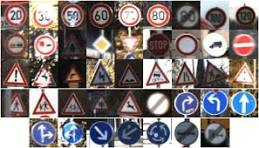
\includegraphics[scale=0.8]{figure2.jpg}
\caption{Some images used in the German Traffic Signs Recognition Benchmark}
\end{figure}

\tab When it comes to the properties used for verifing the network, we can find them in the name of the files which end with the '.vnnlib' extension. They have a specific pattern which contains the description of the image used for that particular verification.

\begin{figure}[h]
\centering
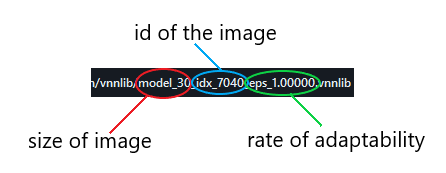
\includegraphics[scale=0.8]{figure3.png}
\caption{Properties file used for verification}
\end{figure}
\tab In the figure above we can see that each file has 3 types of properties, where:
\begin{itemize}
    \item model (red) is defining the size of the image
    \item idx (blue) is the id generated for that specific image
    \item eps (green) is defining the adaptation rate (possible perturbation)
\end{itemize}

\chapter{Tools}
\section{alpha-beta-CROWN}
\tab alpha-beta-CROWN is a neural network verifier based on an efficient linear bound propagation framework and branch and bound, it can provide provable robustness guarantees against adversarial attacks and can also verify other general properties of neural networks\cite{alpha-beta-crown-git}.

\tab For the installation of the alpha-beta-CROWN, we have used the step by step "Instructions for running the VNN-COMP benchmarks"\cite{alpha-beta-instructions} published by the tool developers which contains everything required for a successful installation. Firstly we cloned the git project recursively which also cloned auto\_LiRPA\cite{auto_lirpa_repo} to also support a wide range of neural network architectures.

After having the project locally, we installed Miniconda\cite{miniconda} to be able to have a fresh environment in which we can install the dependencies and run the tool on our benchmark. Here we ran into our first problem, which appeared to be that when trying to create the environment with Miniconda\cite{miniconda}, the yaml extension file defined to specify the dependencies when creating the environment, was containing a redirection to another yaml extension file. The specified redirection did not work and we had to move the dependencies from the redirected yaml extension file to the main yaml extension file.

Once we successfully used the correct yaml file for environment configuration, we ran into our second problem, which was the fact that not all of the dependencies used for alpha-beta-CROWN are available for Windows, therefore we had to change the operating system to a Linux based one and try again.

Finally, when we retried all of the steps with the adaptations written above, the installation was successful and the environment was ready for running benchmarks.

A problem that we encountered on the journey after the installation, was that each time we started the environment, we had to redefine the system variable VNNCOMP\_PYTHON\_PATH which contains the path to python, otherwise the run was not possible to start.

\newpage
\section{Marabou}
\tab The following tool we chose is Marabou\cite{marabou-repository}. Following the GitHub guide, we encountered errors regarding dependant tools that needed to be installed first (more specifically, Pybind11, Protobuf, openBlass, Boost, and Onnx). Due to these issues, we had to find an alternative way to install this tool. That is when we found another solution\cite{marabou-guide}, in which the steps were presented differently, steps which we found were right for our case.\\
\tab The steps are as follows: clone the Marabou repository, install cmake, python and pip, make a build folder and go into it, and from there execute two cmake build instructions. Despite taking some time, the instructions executed successfully, building the Marabou executable, the python package and also numerous testing files for checking the integrity of the tool. This way, we managed to successfully install the tool.\\

\section{Nnenum}
\tab After Marabou, which we could not successfully run, we found another tool: Nnenum\cite{nnenum-repository}. We decided to try it and see if we had better success. And so, we followed the repository instructions, which were a lot easier to go through. All we needed to do is install docker and then run a build docker command with the provided Dockerfile in the repository, and then run the container after the successful build.\\
\tab Fortunately, the repository instructions were correct, and we were able to run the tool. Therefore, we again ran the tool with an onnx and vnnlib file and see the result. Unfortunately, the tool could not implement the operations of Transpose and Sign, two instructions that were present in the onnx files.

\chapter{Experimental results}
\tab When it comes on running the benchmark, we have reached the conclusion that the first benchmark, tllverifybench\cite{tll_verify_bench}, was too simple and flawless to be able to extend the project after a simple run that reproduced the exact output from the competition. Therefore we chose to change it to Traffic Signs Recognition\cite{traffic_signs_recognition} so we can try to solve some of the problems that the competition run had, where we achieved the following values:

\begin{center}
\begin{tabular}{ c c c c c c}
 \hline
 \textbf{\#} & \textbf{Tool} & \textbf{Verified} & \textbf{Falsified} & \textbf{Penalty}\\
 \hline
 1 & alpha-beta-CROWN & 0 & 39 & 3\\
 \hline
 2 & Marabou & - & - & -\\
 \hline
 3 & Nnenum & 0 & 0 & 46\\
 \hline
\end{tabular}
\end{center}

\section{alpha-beta-CROWN}
\tab After the first run we observed that due to a timeout after an instance that timed out, we could not reproduce the exact output due to the process stopping at that point, generating the report only to that specific instance (see

results\_traffic\_signs\_recognition\_default\_time.csv\cite{traffic_signs_recognition_first_solution}). After increasing the timeout in run\_all\_categories.sh file found in the alpha-beta-CROWN project, we were able to reproduce the output, but the instance that crashed the process still timed out, this time after 1000.0 seconds (the given value, see

results\_traffic\_signs\_recognition\_increased\_time\_to\_1000.csv\cite{traffic_signs_recognition_second_solution}).\\

\begin{figure}[h]
\centering
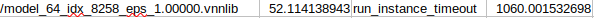
\includegraphics[scale=0.6]{run_instance_timeout.png}
\caption{Run instance timeout of a specific network ran with displayed properties}
\end{figure}

The falsified responses comes from the fact that, the output for most of the instances, seem to be satisfiable when in fact there is still generated an counter-example for 39 of the instances which turn to be a false positive. The penalty comes from 3 instances that have the result different than "sat" or "unsat". Two of them have the result "no\_result\_in\_file" and after having a look in the logs, it appears that the branch-and-bound (BaB) round 69 stops (kills) the process in both instances therefore there is no output file from which to get the result. No successful method in changing the BaB and timeout configurations was found yet after some failed attempts.

The remaining instance that fails with the "run\_instance\_timeout" seems to not be fixed after increasing the timeout from 480 seconds to 1000, further timeout increase will be made to test if any real timeout value can fix the problem.

\section{Marabou}
\tab We have tried to take an example onnx and vnnlib property file from the traffic sign benchmark dataset and run the executable with it. Unfortunately we encountered a Segmentation Fault error. We also tried to run the python program with the same arguments, but we also encountered errors. Without many tools online to solve this problem, we were left with the option to try another tool and see if we would have better success with it.

\section{Nnenum}
\tab As a final tool experiemntal run, we have tried Nnenum and went to the vnncomp-2023 folder and ran all the instances for the traffic sign recognition dataset, and we did get an out.csv file where we had exit code of 1 instead of actual results, but with a runtime value. Despite this setback, this was an easier tool to run and we did get an improvement over the previous one.

\chapter{Conclusions}
\tab In conclusion, it seems that the dataset Traffic Signs Recognition\cite{traffic_signs_recognition} it is very hard to be verified 100\% because even if a small adaptation rate (epsilon) like 1.00, the image will differ unless we set an adaptation rate of 0. Beside of this, all of the tools found penalties for this dataset for some verification cases which had a small adaptation rate number (1.00 and 5.00) which indicates that for those cases the image could not be verified unless we increase the specified rate.\\
\tab Nonetheless, it seems that the possibility of improving the benchmark and the tools is present, because in our case there could be chosen other images for those specific signs that fail on which the adaptation rate would not be necesary to be higher to be verified. On the tools side, alpha-beta-CROWN is much more friendlier for anyone to run either the competition benchmark, or any benchmark needed, by offering more clearer documentation on how to do it. When trying to experiment the same with Marabou, it only has the support for 2 benchmarks, none of them being our benchmark.

\bibliography{references}
\bibliographystyle{alpha}
\end{document} 